\documentclass[11pt,a4paper]{book}

\usepackage{Appunti}

\begin{document}
\title{Clean Code\\
\large{\textit{Robert C. Martin}}}
\author{Jacopo De Angelis}
\maketitle

\pagebreak
\tableofcontents
\pagebreak

\chapter{Clean code}
Il codice non finirà con l'era dell'autogenerazione da IA. Qualcuno dovrà creare le IA, qualcuno dovrà imparare come dare le specifiche. Il codice sarà sempre presente.

\section{Pessimo codice}
Una delle prime cause del pessimo codice è la fretta dettata dall'ansia. L'idea di dover far uscire il codice il prima possibile ci porta a commettere errori, commettere inesattezze. Quello è ciò che può portare a seri problemi successivamente, il rileggere il proprio codice scritto in maniere quantomeno esecrabili è una tortura. E ricordiamo che se si pensa "lo metto a posto dopo", dopo equivale a mai.

I rallentamenti derivanti da nuovo codice di bassa qualità sono esponenziali, lentamente la produttività crolla perchè operare sul codice precedente è sempre più complicato.
\begin{figure}[h!]
	\begin{center}
		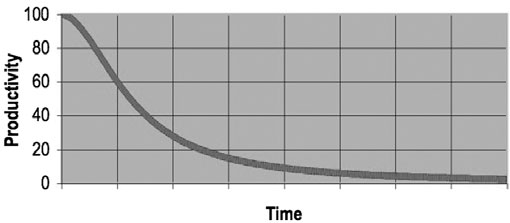
\includegraphics[scale=0.6]{img/001.png}
		\caption{Produttività vs tempo}
		\label{fig: 001}
	\end{center}
\end{figure}

Il che può portare ad un desiderio di ricreare da zero l'intera base del codice, cosa non solo dispendiosa ma che richiede anche molto tempo. I team si trovano a lavorare in parallelo, il nuovo team che ricrea tutto e integra il nuovo lavoro del vecchio team e, alla fine, ci si troverà nella stessa situazione.

\section{Scrivere buon codice}
Scrivere buon codice richiede disciplina nell'uso di molte piccole tecniche applicate in ogni singolo momento. Tutto questo richiede anche una parte di "senso estetico", un percepire il perchè un bel codice sia, appunto, bello.

Una regola che possiamo ereditare dai boy scout: lascia il campo più pulito di come l'hai trovato. Ad esempio: una variabile può avere un nome più autoesplicativo? Cambiala. Una funzione può essere spezzata in più funzioni elementari? Dividila.

\chapter{Nomi significativi}
\section{Usare nomi che rivelino l'intenzione}
Trovare nomi significativi non è semplice ma il tempo che prendono nel farlo è sicuramente meno di quello speso a decifrare nomi non chiari.

Ogni nome, che sia di variabile o di funzione, deve rispondere alle domande:
\begin{itemize}
	\item[] Cosa fa
	\item[] Perchè esiste
	\item[] Come viene utilizzata
\end{itemize}
Se un nome richiede un commento allora il nome è sbagliato.

Ad esempio
\lstinputlisting[language=]{code/001}\label{code: 001}
d non dice molto come nome. Dovremmo scegliere un nome migliore, ad esempio
\lstinputlisting[language=]{code/002}\label{code: 002}
Scegliere un nome che rivela un intento rende molto più semplice cambiare e comprendere un codice. Ad esempio cosa fa questo pezzo di codice?
\lstinputlisting[language=]{code/003}\label{code: 003}
Il problema di questo codice non è la sua semplicità ma la sua capacità di avere un senso implicito. Ad esempio, le domande che ci possiamo porre sono:
\begin{itemize}
	\item[] Cos'è theList?
	\item[] Che significato ha l'elemento 0 di theList?
	\item[] Qual è il significato di 4?
	\item[] Come viene usata la lista ritornata?
\end{itemize}

Queste risposte dovrebbero essere nel codice. Immaginiamo ora di lavorare a campo minato. Rinominiamo la lista con gameBoard.

Ogni cella della board è rappresentata da un array, il valore alla posizione 0 è la posizione dello status della cella e se è 4 vuol dire "segnata". Già dando implicitamente queste notazioni possiamo migliorare il codice:
\lstinputlisting[language=]{code/004}\label{code: 004}

Possiamo andare anche oltre e scrivere una semplice classe per le celle invece di avere degli int. Può includere una funzione con un nome che ne sveli l'intento per nascondere questo numero. Il risultato è:
\lstinputlisting[language=]{code/005}\label{code: 005}

\section{Evitare la disinformazione}

\end{document}